\section{Auswertung}

\subsection{Untersuchung eines Acrylblocks \label{sec:acryl}}

\subsubsection{A-Scan \label{sec:ascan}}

In Tabelle \ref{tab:ascan} befinden sich die aufgenommenen und berechneten Werte.
\begin{table}[H]
   \centering
   \caption{Die mithilfe des A-Scans aufgenommenen und berechneten Werte}
   \label{tab:ascan}
   \makebox[1 \textwidth][c]{       %centering table
   \begin{tabular}{ c S S S S S S S }
 \toprule
 {Lochnummer} & {$d_\text{theo}\:/\: \mathrm{cm}$} & {$t_\text{oben}\:/\: \symup{\mu s}$} & {$s_\text{oben}\:/\: \mathrm{mm}$} &
 {$t_\text{unten}\:/\: \symup{\mu s}$} & {$s_\text{unten}\:/\: \mathrm{mm}$} & {$d\:/\: \mathrm{mm}$} & {Abweichung} \\
    \midrule
    3 & 0,6 & 46,34 & 61,25 & 11,00 & 13,01 & 5,73 & 4,48\% \\
    4 & 0,5 & 40,63 & 53,46 & 17,14 & 21,40 & 5,14 & 2,88\% \\
    5 & 0,4 & 35,23 & 46,09 & 23,91 & 30,64 & 3,27 & 18,15\% \\
    6 & 0,3 & 29,84 & 38,73 & 29,73 & 38,58 & 2,69 & 10,43\% \\
    7 & 0,2 & 23,70 & 30,35 & 35,55 & 46,53 & 3,12 & 56,19\% \\
    8 & 0,2 & 18,09 & 22,69 & 41,58 & 54,76 & 2,55 & 27,52\% \\
    9 & 0,2 & 12,17 & 14,61 & 47,19 & 62,41 & 2,97 & 48,68\% \\
    10 & 0,2 & 6,35 & 6,67 & 53,33 & 70,80 & 2,54 & 26,84\% \\
    11 & 0,9 & 42,22 & 55,63 & 12,49 & 15,05 & 9,32 & 3,57\% \\
    \bottomrule
  \end{tabular}
  }
\end{table}


Die Werte für $s_\text{oben}$ und $s_\text{unten}$ ergeben sich aus \eqref{eqn:s}
\begin{equation}
  s = \frac{1}{2} \cdot c_\text{Acryl} \cdot t - \xi.
  \label{eqn:s}
\end{equation}
\begin{center}
 \tiny{($c_\text{Acryl} = \SI{2730}{\m \per \s}$ \cite{sample2}, $\xi = \SI{0,2}{\cm} \: \hat{=} \: \text{Anpassungsschicht der Ultraschallsonde}$)}
\end{center}

Die Dicke der Fehlstellen berechnet sich aus \eqref{eqn:d}
\begin{equation}
  d = h - s_\text{oben} - s_\text{unten}.
  \label{eqn:d}
\end{equation}
\begin{center}
 \tiny{($h = \SI{8}{\cm} \: \hat{=} \: \text{Höhe des Zylinders}$)}
\end{center}

\subsubsection{B-Scan \label{sec:bscan}}

In Abbildung \ref{fig:bscan} befinden sich die beiden aufgenommenen B-Scans.
\begin{figure}[H]
  \caption{Mit dem B-Scan untersuchter Acrylblock}
  \label{fig:bscan}
  \centering
        \begin{subfigure}[b]{\textwidth}
                \centering
                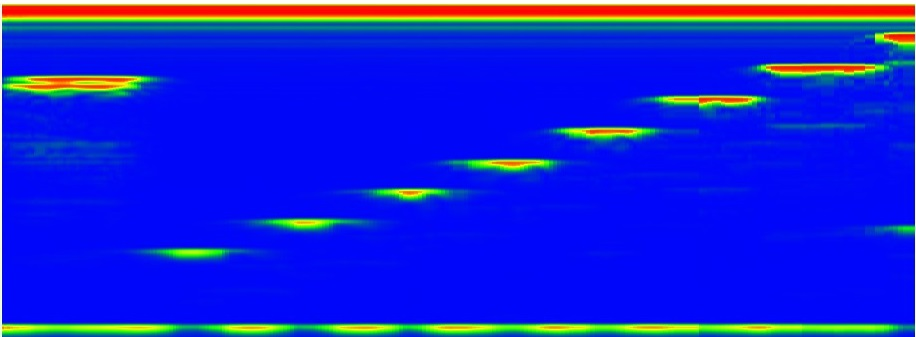
\includegraphics[width=\textwidth]{Scan-Bilder/bscanoben.jpg}
                \caption{Acrylblock von oben mit einer $\SI{2}{\MHz}$-Sonde}
                \label{fig:oben}
        \end{subfigure}
        \quad
        \begin{subfigure}[b]{\textwidth}
                \centering
                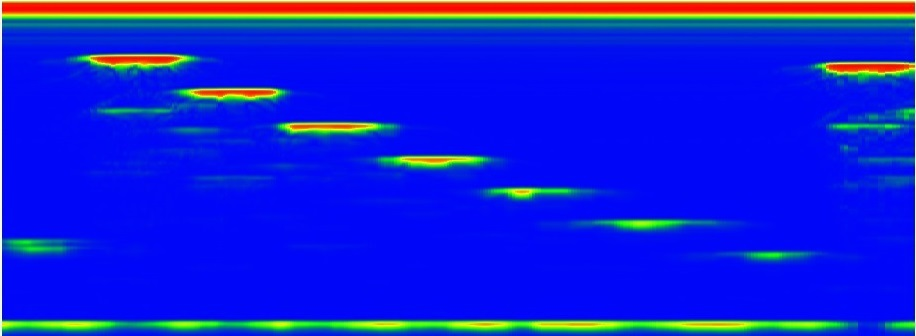
\includegraphics[width=\textwidth]{Scan-Bilder/bscanunten.jpg}
                \caption{Acrylblock von unten mit einer $\SI{2}{\MHz}$-Sonde}
                \label{fig:unten}
        \end{subfigure}
\end{figure}

In Tabelle \ref{tab:bscan} befinden sich die aufgenommenen und berechneten Werte
\begin{table}[H]
   \centering
   \caption{Die mithilfe des B-Scans aufgenommenen und berechneten Werte}
   \label{tab:bscan}
   \begin{tabular} { c *5{S} }
 \toprule
 {Lochnummer} & {$d_\text{theo}\:/\: \mathrm{cm}$} & {$t_\text{oben}\:/\: \symup{\mu s}$} & {$t_\text{unten}\:/\: \symup{\mu s}$} &
 {$d\:/\: \mathrm{mm}$} & {Abweichung} \\
    \midrule
    3 & 0,6 & 45,93 & 10,74 & 6,65 & 10,83\% \\
    4 & 0,5 & 40,37 & 16,85 & 5,89 & 17,83\% \\
    5 & 0,4 & 34,81 & 23,15 & 4,88 & 22,01\% \\
    6 & 0,3 & 29,44 & 29,44 & 3,62 & 20,56\% \\
    7 & 0,2 & 23,52 & 35,19 & 3,87 & 93,47\% \\
    8 & 0,2 & 17,78 & 41,11 & 3,62 & 80,83\% \\
    9 & 0,2 & 11,85 & 47,04 & 3,62 & 80,83\% \\
    10 & 0,2 & 6,11 &  &  &  \\
    11 & 0,9 & 41,67 & 12,22 & 10,44 & 16,02\% \\
    \bottomrule
  \end{tabular}
\end{table}


Die Werte für $s_\text{oben}$, $s_\text{unten}$ und $d$ ergeben sich wie in Kapitel \ref{sec:ascan} aus den Gleichungen \eqref{eqn:s}
und \eqref{eqn:d}.

\subsection{Untersuchung des Auflösungsvermögens \label{sec:auf}}

In Abbildung \ref{fig:auf} befinden sich die mit unterschiedlichen Sonden aufgenommenen A-Scans.
\begin{figure}[H]
  \caption{A-Scans mithilfe unterschiedlicher Ultraschallsonden von Loch 1 und 2}
  \label{fig:auf}
  \centering
  \makebox[1 \textwidth][c]{
        \begin{subfigure}[b]{0.69\textwidth}
                \centering
                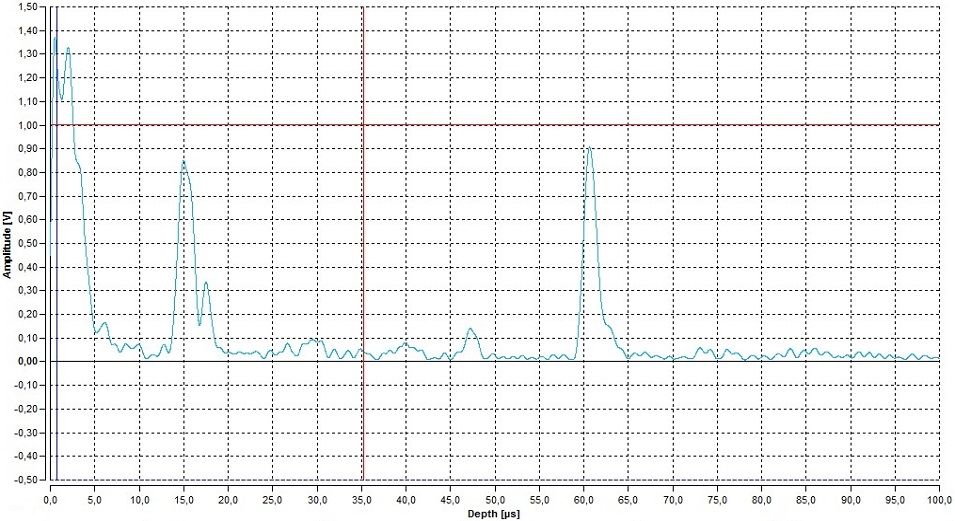
\includegraphics[width=\textwidth]{Scan-Bilder/aufblau.jpg}
                \caption{$\SI{1}{\MHz}$-Sonde}
                \label{fig:blau}
        \end{subfigure}
        \quad
        \begin{subfigure}[b]{0.69\textwidth}
                \centering
                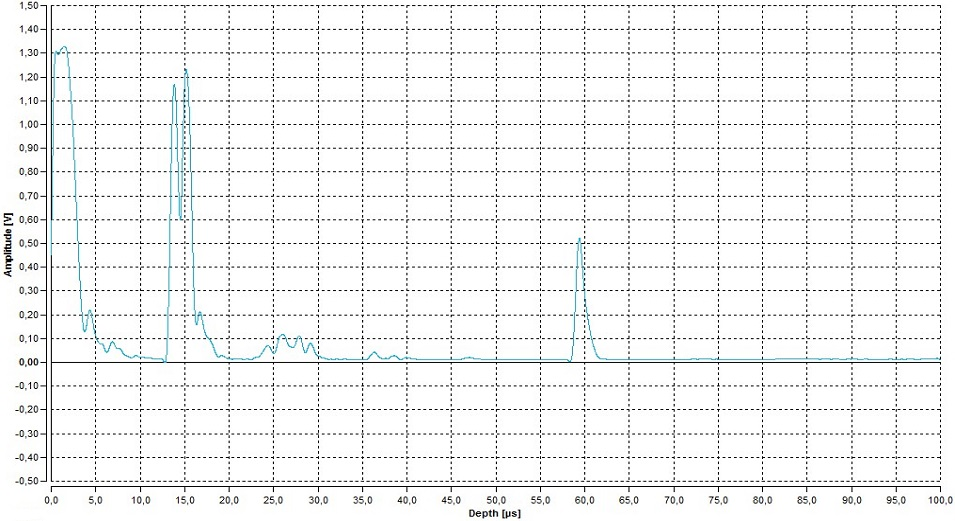
\includegraphics[width=\textwidth]{Scan-Bilder/aufrot.jpg}
                \caption{$\SI{2}{\MHz}$-Sonde}
                \label{fig:rot}
        \end{subfigure}
        }
        \par\bigskip
        \begin{subfigure}[b]{0.69\textwidth}
                \centering
                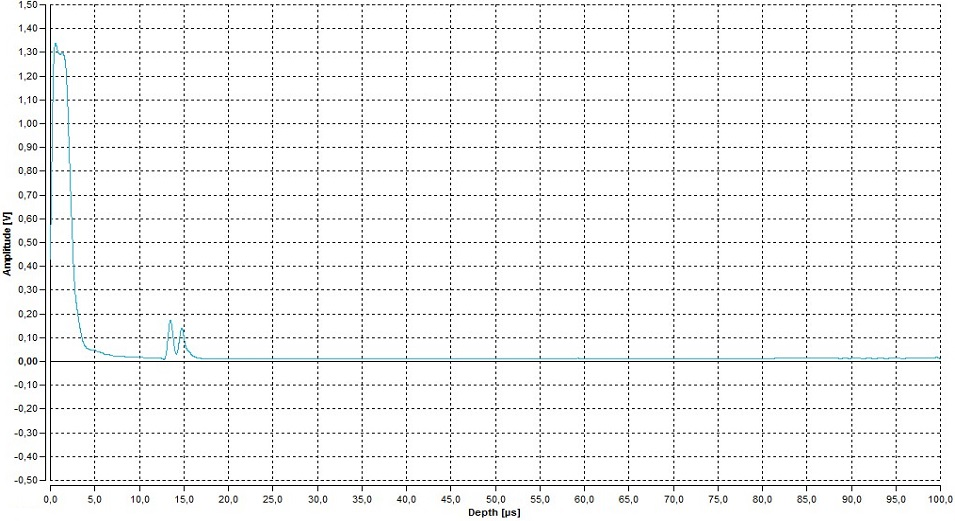
\includegraphics[width=\textwidth]{Scan-Bilder/aufgruen.jpg}
                \caption{$\SI{4}{\MHz}$-Sonde}
                \label{fig:grün}
        \end{subfigure}
\end{figure}

Bei der $\SI{4}{\MHz}$-Sonde werden die Schallwellen zu stark vom Material geschwächt, sodass das Signal kaum erkennbar ist.
Die $\SI{1}{\MHz}$-Sonde liefert eine ordentliche Auflösung, allerdings sind die beiden Peaks etwas kleiner als
bei der $\SI{2}{\MHz}$-Sonde. Dies liegt daran, dass bei dieser Frequenz die Wellenlänge der Schallwellen ungefähr der Größenordnung
der Lochdurchmesser entspricht.

\subsection{Untersuchung eines Herzmodells mit dem TM-Scan}

In Abbildung \ref{fig:herz} befindet sich der aufgenommene TM-Scan.
\begin{figure}[H]
  \centering
  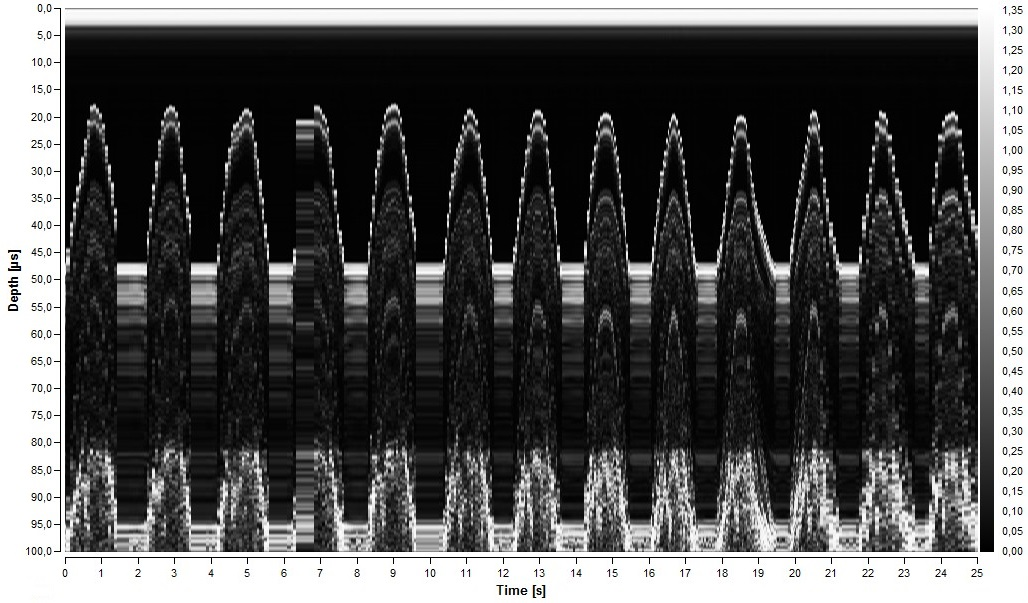
\includegraphics[width=\textwidth]{Scan-Bilder/tmscan0.jpg}
  \caption{TM-Scan des Herzmodells}
  \label{fig:herz}
\end{figure}

In Tabelle \ref{tab:herz} befinden sich die aus Abbildung \ref{fig:herz} abgelesenen Werte.
\begin{longtable}{ c c c S S S }
  \caption{Aufgenommene Messwerte des Rhodium-Zerfalls unter Berücksichtigung des Nulleffekts mit der berechneten Logarithmierung und ihren Abweichungen}
  \label{tab:rhod} \\
  \toprule
  {$t\:/\: \mathrm{s}$} & {$N$} & {$N\:/\: \mathrm{Bq}$} & {$\ln{(N)}$} & {$\ln{(N+\sigma)}-\ln{(N)}$} & {$\ln{(N)}-\ln{(N-\sigma)}$} \\
  \midrule
 \endfirsthead
  \caption{Aufgenommene Messwerte des Rhodium-Zerfalls unter Berücksichtigung des Nulleffekts mit der berechneten Logarithmierung und ihren Abweichungen (Fortsetzung)} \\
 \toprule
 {$t\:/\: \mathrm{s}$} & {$N$} & {$N\:/\: \mathrm{Bq}$} & {$\ln{(N)}$} & {$\ln{(N+\sigma)}-\ln{(N)}$} & {$\ln{(N)}-\ln{(N-\sigma)}$} \\
  \midrule
 \endhead
  \midrule
 \endfoot
  \bottomrule
 \endlastfoot
    18 & 602 & 33,19\pm1,36 & 3,50 & 0,04 & 0,04 \\
    36 & 507 & 27,92\pm1,25 & 3,33 & 0,04 & 0,05 \\
    54 & 371 & 20,36\pm1,06 & 3,01 & 0,05 & 0,05 \\
    72 & 297 & 16,25\pm0,95 & 2,79 & 0,06 & 0,06 \\
    90 & 232 & 12,64\pm0,84 & 2,54 & 0,06 & 0,07 \\
    108 & 201 & 10,92\pm0,78 & 2,39 & 0,07 & 0,07 \\
    126 & 172 & 9,31\pm0,72 & 2,23 & 0,07 & 0,08 \\
    144 & 115 & 6,14\pm0,58 & 1,81 & 0,09 & 0,10 \\
    162 & 122 & 6,53\pm0,60 & 1,88 & 0,09 & 0,10 \\
    180 & 87 & 4,58\pm0,50 & 1,52 & 0,10 & 0,12 \\
    198 & 79 & 4,14\pm0,48 & 1,42 & 0,11 & 0,12 \\
    216 & 57 & 2,92\pm0,40 & 1,07 & 0,13 & 0,15 \\
    234 & 74 & 3,86\pm0,46 & 1,35 & 0,11 & 0,13 \\
    252 & 57 & 2,92\pm0,40 & 1,07 & 0,13 & 0,15 \\
    270 & 55 & 2,81\pm0,39 & 1,03 & 0,13 & 0,15 \\
    288 & 46 & 2,31\pm0,36 & 0,84 & 0,14 & 0,17 \\
    306 & 50 & 2,53\pm0,37 & 0,93 & 0,14 & 0,16 \\
    324 & 40 & 1,97\pm0,33 & 0,68 & 0,16 & 0,18 \\
    342 & 48 & 2,42\pm0,37 & 0,88 & 0,14 & 0,16 \\
    360 & 32 & 1,53\pm0,29 & 0,42 & 0,17 & 0,21 \\
    378 & 40 & 1,97\pm0,33 & 0,68 & 0,16 & 0,18 \\
    396 & 34 & 1,64\pm0,30 & 0,49 & 0,17 & 0,20 \\
    414 & 31 & 1,47\pm0,29 & 0,39 & 0,18 & 0,22 \\
    432 & 16 & 0,64\pm0,19 & -0,45 & 0,26 & 0,35 \\
    450 & 26 & 1,19\pm0,26 & 0,18 & 0,20 & 0,24 \\
    468 & 38 & 1,86\pm0,32 & 0,62 & 0,16 & 0,19 \\
    486 & 25 & 1,14\pm0,25 & 0,13 & 0,20 & 0,25 \\
    504 & 34 & 1,64\pm0,30 & 0,49 & 0,17 & 0,20 \\
    522 & 34 & 1,64\pm0,30 & 0,49 & 0,17 & 0,20 \\
    540 & 25 & 1,14\pm0,25 & 0,13 & 0,20 & 0,25 \\
    558 & 20 & 0,86\pm0,22 & -0,15 & 0,23 & 0,29 \\
    576 & 23 & 1,03\pm0,24 & 0,03 & 0,21 & 0,26 \\
    594 & 17 & 0,69\pm0,20 & -0,36 & 0,25 & 0,33 \\
    612 & 15 & 0,58\pm0,18 & -0,54 & 0,27 & 0,37 \\
    630 & 24 & 1,08\pm0,25 & 0,08 & 0,20 & 0,26 \\
    648 & 14 & 0,53\pm0,17 & -0,64 & 0,28 & 0,39 \\
    666 & 18 & 0,75\pm0,20 & -0,29 & 0,24 & 0,32 \\
    684 & 22 & 0,97\pm0,23 & -0,03 & 0,21 & 0,27 \\
    702 & 19 & 0,81\pm0,21 & -0,22 & 0,23 & 0,30 \\
    720 & 18 & 0,75\pm0,20 & -0,29 & 0,24 & 0,32 \\
    738 & 20 & 0,86\pm0,22 & -0,15 & 0,23 & 0,29 \\
    756 & 17 & 0,69\pm0,20 & -0,36 & 0,25 & 0,33 \\
    774 & 17 & 0,69\pm0,20 & -0,36 & 0,25 & 0,33 \\
\end{longtable}


Die Mittelwerte und ihre Fehler für $T$ und $h$ betragen
\begin{align*}
  \bar{T} &= \SI{1,99(3)}{\s} \\
  \bar{h} &= \SI{28,42(20)e-6}{\s}
\end{align*}

und ergeben sich aus den Formeln \eqref{eqn:mit} und \eqref{eqn:sta}
\begin{align}
  \bar{x} &= \frac{1}{N} \sum_{i=1}^{N} x_i \label{eqn:mit} \\
  \Delta \bar{x} &= \sqrt{\frac{1}{N (N - 1)} \sum_{i=1}^{N} (x_i - \bar{x})^2}. \label{eqn:sta}
\end{align}

Die Frequenz $\nu$ ergibt sich aus Formel \eqref{eqn:frq}
\begin{equation}
  \nu = \frac{1}{\bar{T}}.
  \label{eqn:frq}
\end{equation}

Den Fehler erhält man aus der Gauß'schen Fehlerfortpflanzung \eqref{eqn:gaus}
\begin{equation}
  \delta = \sqrt{\sum_{i=1}^{n}\left(\frac{\partial y}{\partial x_i} \Delta x_i\right)^2}.
  \label{eqn:gaus}
\end{equation}

Somit ergibt sich für die Herzfrequenz
\begin{equation*}
  \nu_\text{Herz} = \SI{0,502(9)}{\Hz}.
\end{equation*}

Mithilfe von Gleichung \eqref{eqn:s} und der Gauß'schen Fehlerfortpflanzung \eqref{eqn:gaus} lässt sich der Höhenunterschied $s$ zwischen
der Systole und der Diastole zu
\begin{equation*}
  s = \SI{2,11(2)}{\cm}
\end{equation*}
bestimmen.

Das Schlagvolumen $V$ ergibt sich aus der Formel für das Volumen eines Kugelsegments und der Gauß'schen Fehlerfortpflanzung \eqref{eqn:gaus}
\begin{equation*}
  V = \frac{s \cdot \pi}{6} \cdot \left(3a^2 + s^2 \right)= \SI{25,6(3)}{\ml}.
  \label{eqn:vol}
\end{equation*}
\begin{center}
  \tiny{($a = \SI{2,5}{\cm} \: \hat{=} \: \text{Radius des Herzmodells}$)}
\end{center}

Nun lässt sich mit Gleichung \eqref{eqn:gaus} das Herzzeitvolumen $HZV = V \cdot \nu_\text{Herz}$ berechnen
\begin{equation*}
  HZV = \SI{12,8(3)}{\ml \per \s} = \SI{0,77(2)}{\l \per \min}.
\end{equation*}
